\subsection{个人贷款统计问题}
具体问题描述可见 \ref{pro4} 个人贷款统计问题一节.

备注:此case1我们花了一定时间,没有通过评测。最初其结果集有误,后续赛事组才进行
修改,我们当时忙于处理case4,遂对该题没有过多的深入。

此问题涉及的数据文件有:
\begin{itemize}
  \item Person.csv(点)
  \item Account.csv(点)
  \item Loan.csv(点)
  \item AccountTransferAccount.csv(边)
  \item LoanDepositAccount.csv(边)
  \item PersonOwnAccount.csv(边)
\end{itemize}

\subsubsection{思路历程}
根据题目需分三步走,逐步将loan值往前传。首先导入account点和loan点,
通过loandepositaccount的边和其值amout创建一张图,向前传递amount值;再将上一步
生成的含有accountid和value的表与accounttransferaccount的边结合生成一张图,将value
的值向前传递;最后将上一步生成的含有accountid和value的表与personownaccount边、
person点相结合,向前传递value值实现个人贷款的汇总。

\subsubsection{代码分析与实现}
运用赛题所给的接口,我们先将account和loan都当作点,点的id即为account或loan对应
的id,将account的初始value设为0,将loan的初始value设为-1(方便后续筛选);而对
于边,我们将loandepositaccount的amount设为其边的value,两侧点按顺序填入相应的id,
通过输入流pwindowsource分别进行输入。接着我们用buildwindowstreamgraph进行构图,
在构图中我们用union操作将loan和account点合并在一起。考虑到loan和account的id有重
复的部分(通过set检测,遍历两个文件后统计数量是否变化),由于loan点在后续代码中
并没有使用,因此在loan点的id前加入字符“l”以进行区分,防止account之间或者loan
之间的相连。代码如下:
\begin{figure}[H]
  \begin{center}
    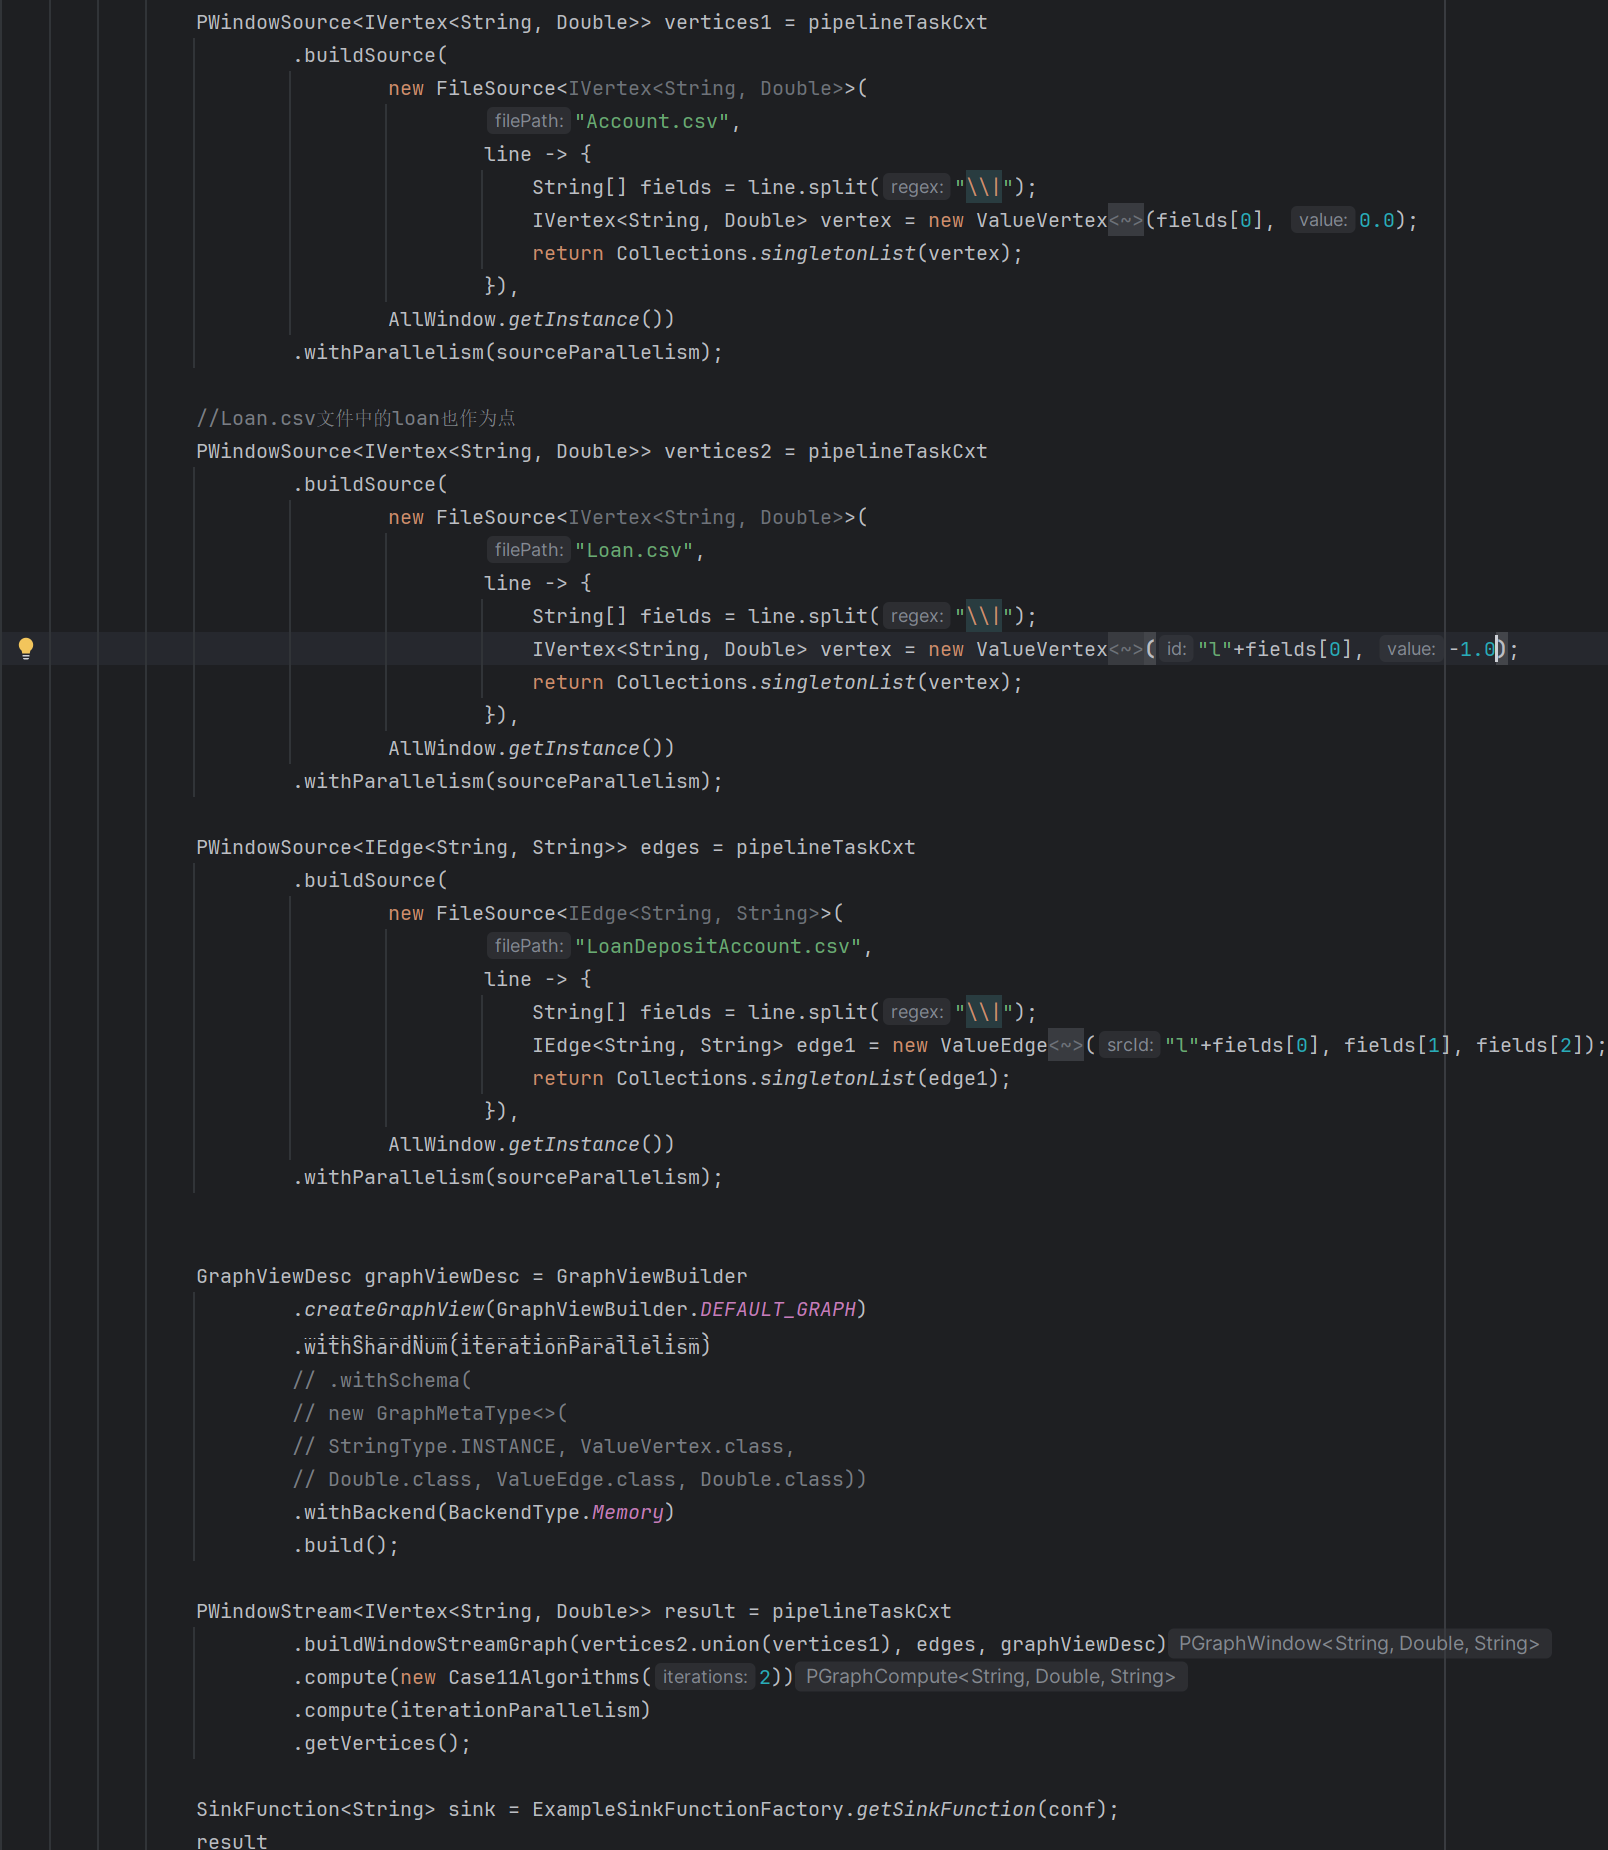
\includegraphics[width=0.85\textwidth,scale=0.7]{./figures/pro4/1.png}
  \end{center}
\end{figure}

接着我们需要得出一个新文件让每个account带上amount,于是,算法思路是进行对所有
点进行两轮迭代,第一轮所有点迭代中,让所有拥有出边的loan点(即此loan有至少一个
账户deposit),向所有出边的目标点(即account点)发送边的amount值。在第二轮迭代
中,由于每个点都有一个接收器,我们让所有接收器不为空的点计算接收器的总和sum并
将value值更新为sum,
到这一步,所有account的value值大于等于 $ 0 $,所有loan的value值都为 $ -1 $,核心代码如下:
\begin{figure}[H]
  \begin{center}
    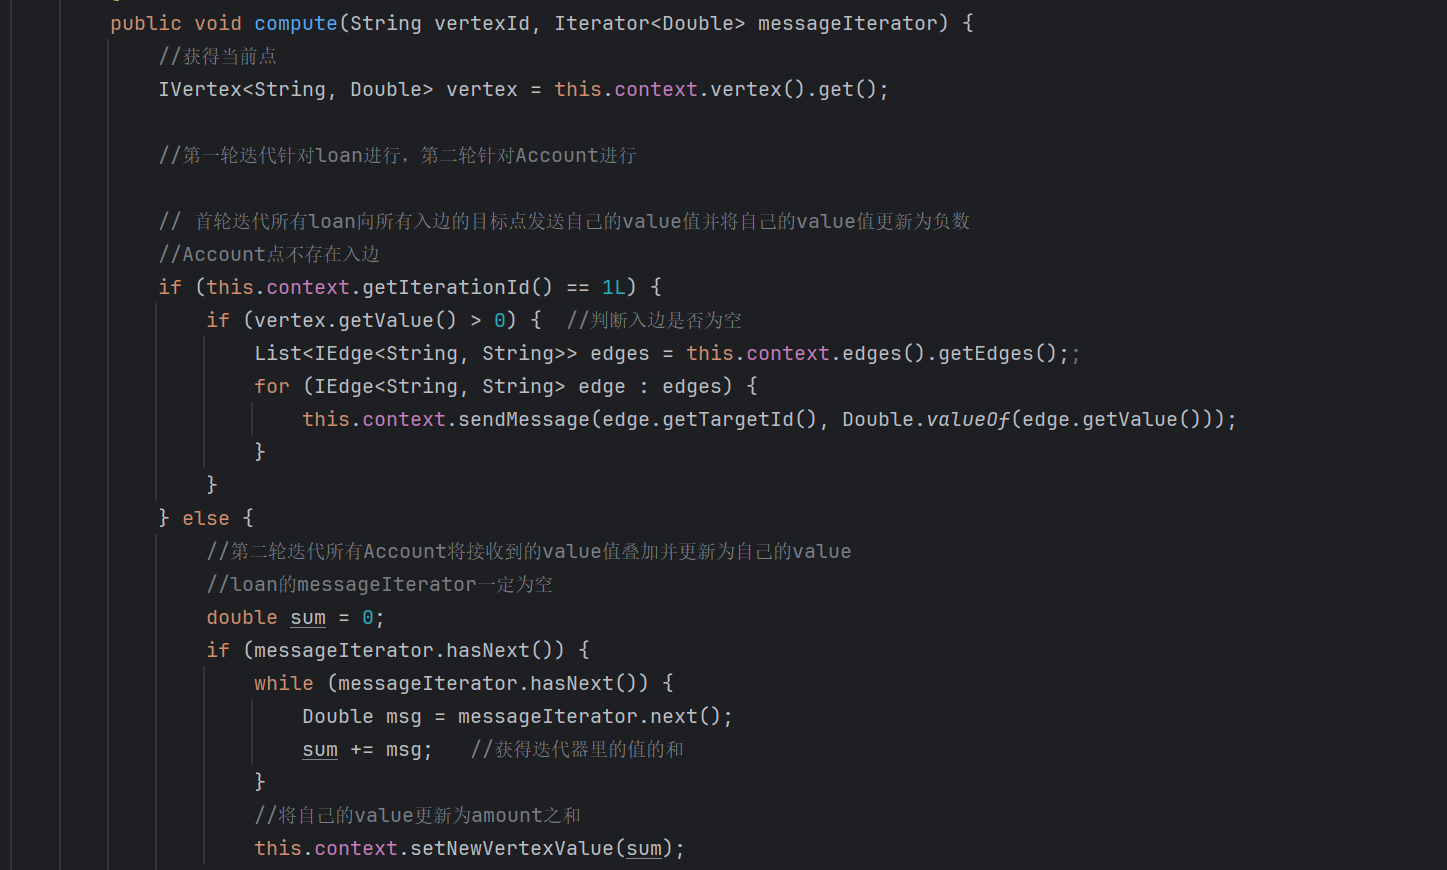
\includegraphics[width=0.85\textwidth,scale=0.7]{./figures/pro4/2.png}
  \end{center}
\end{figure}

最后,将所有点进行过滤涤除value 小于 $ 0 $ 的点(即loan点)得到中间文件。
\begin{figure}[H]
  \begin{center}
    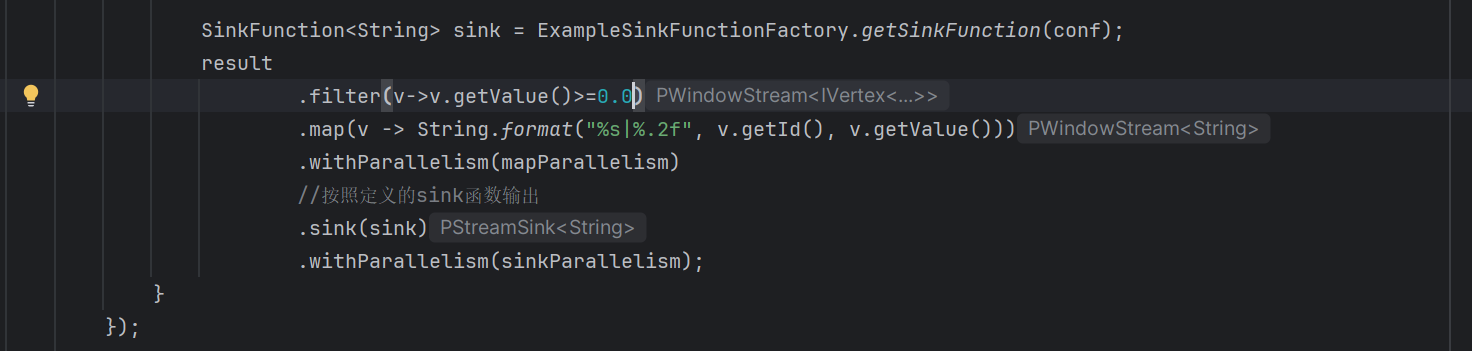
\includegraphics[width=0.85\textwidth,scale=0.7]{./figures/pro4/3.png}
  \end{center}
\end{figure}

接着进入第二步操作,首先我们将中间文件与accounttransferaccount文件联合起来构建成
图,点的id为account的id,点的value为account的value,边的value为空字符串:
\begin{figure}[H]
  \begin{center}
    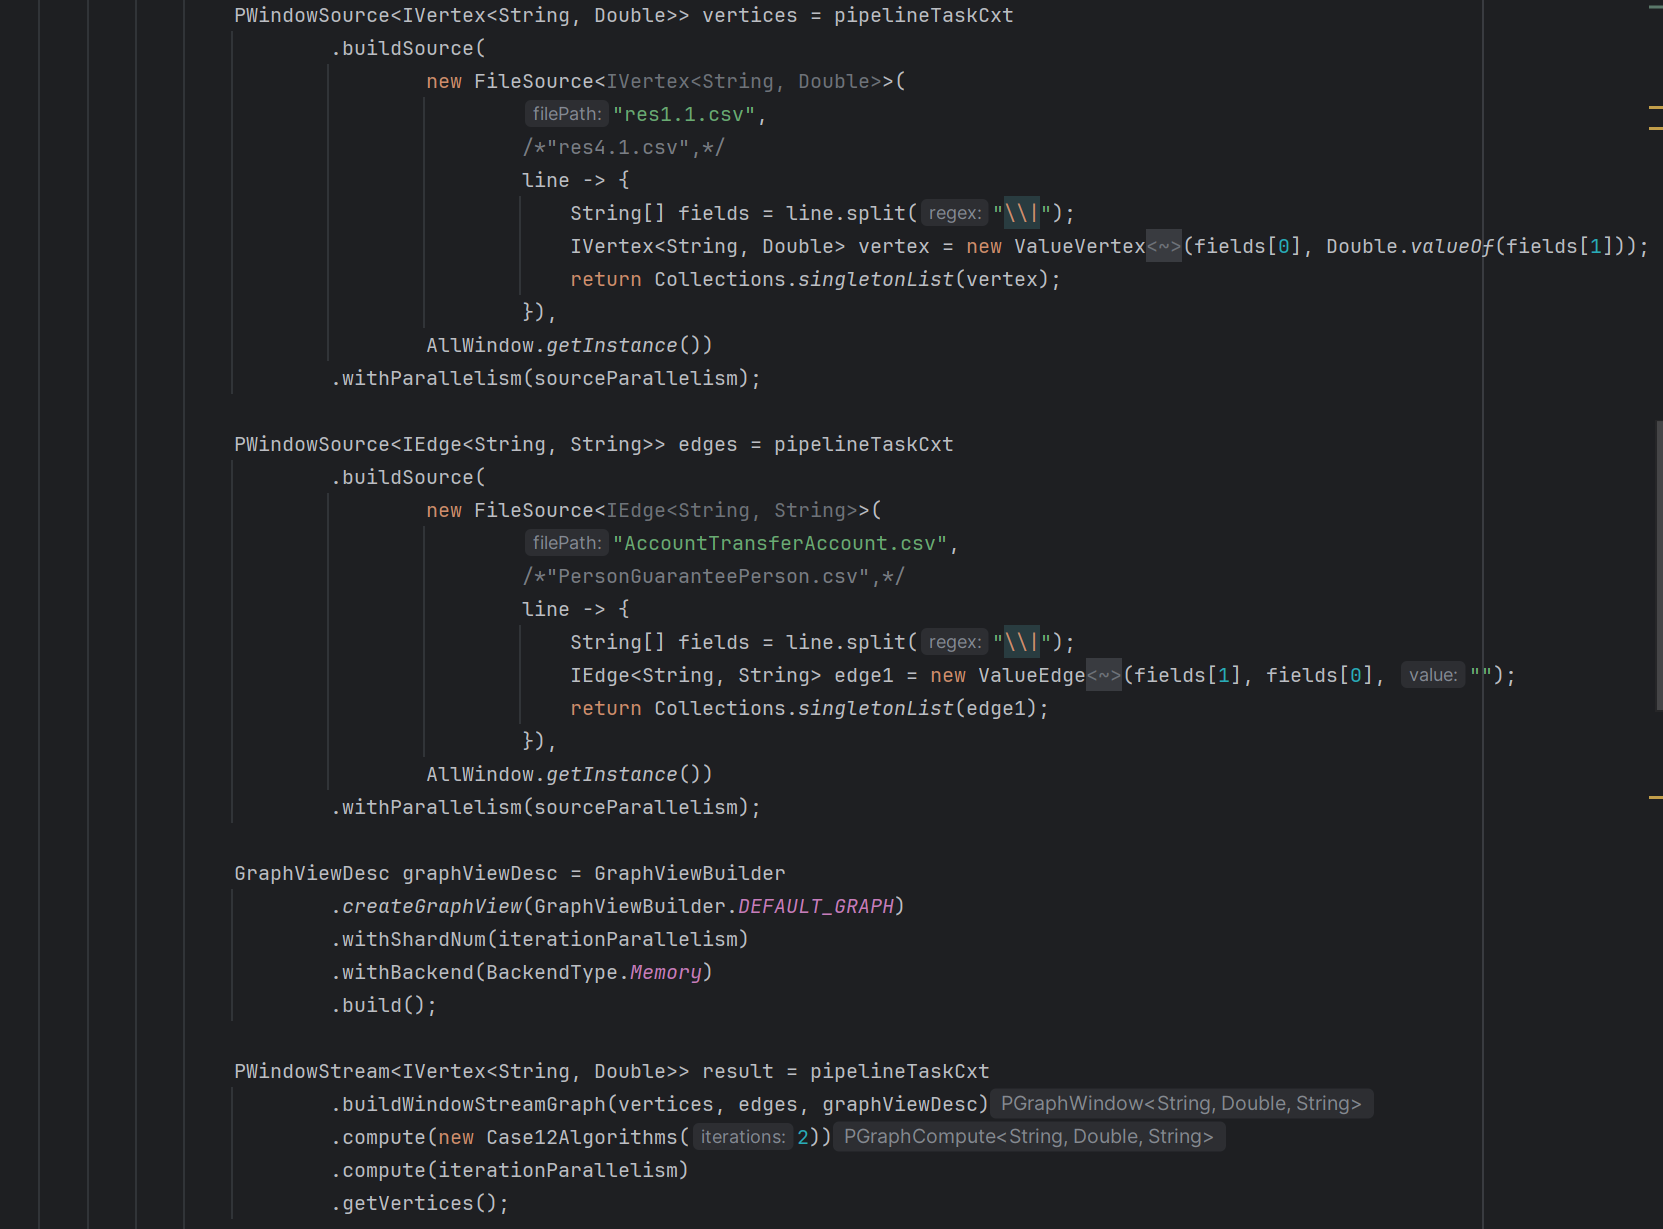
\includegraphics[width=0.85\textwidth,scale=0.7]{./figures/pro4/4.png}
  \end{center}
\end{figure}

接着我们进行两轮迭代,与第一次处理类似,将点的value值根据边往前传递。
需要注意的是,为防止未经过transfer的点在最后一轮也被计算进去,在传递前先让所有点
都向自己的接收器发送0.0(接收器没有值的点不会进入第二轮迭代),并在第二轮迭代中
进行更新value值,这样就只有通过边传递值的account的value值不为0。核心代码如下:
\begin{figure}[H]
  \begin{center}
    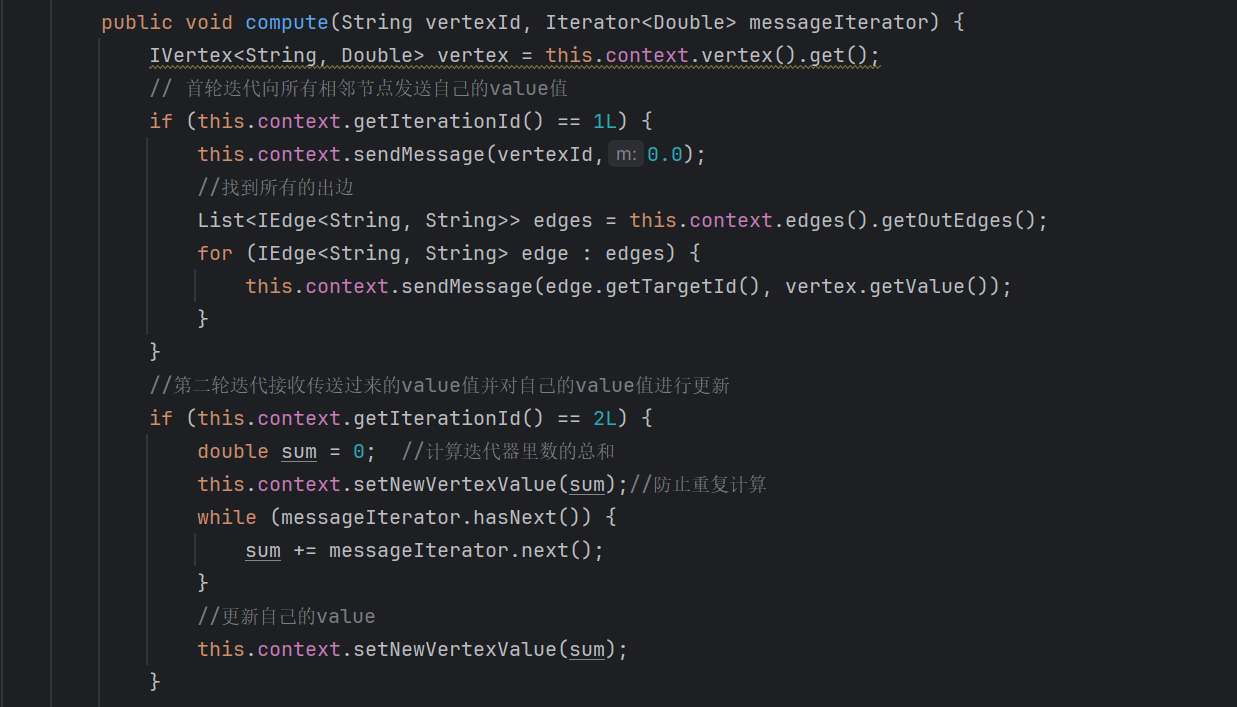
\includegraphics[width=0.85\textwidth,scale=0.7]{./figures/pro4/5.png}
  \end{center}
\end{figure}

第二次中间文件输出格式如下:
\begin{figure}[H]
  \begin{center}
    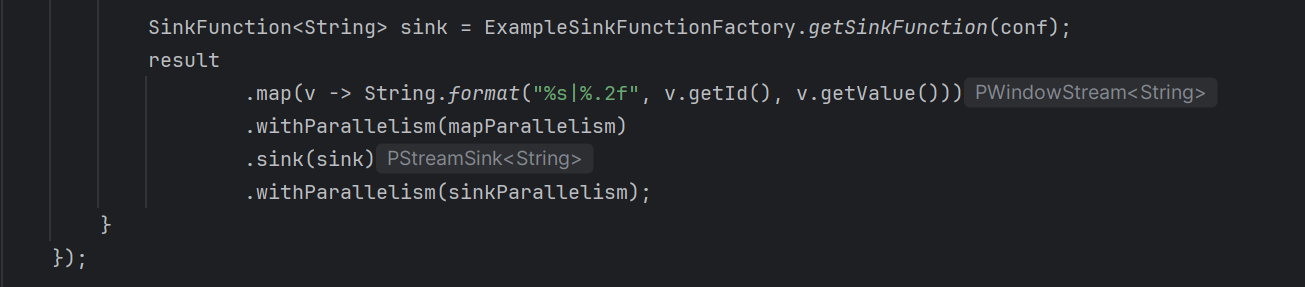
\includegraphics[width=0.85\textwidth,scale=0.7]{./figures/pro4/6.png}
  \end{center}
\end{figure}

接着进入第三步操作,首先我们将中间文件与personownaccount文件和person文件联合起
来构建成图,点的id为account或者person的id,点的value为account的value,person的
value置为0,边的value为空字符串:
\begin{figure}[H]
  \begin{center}
    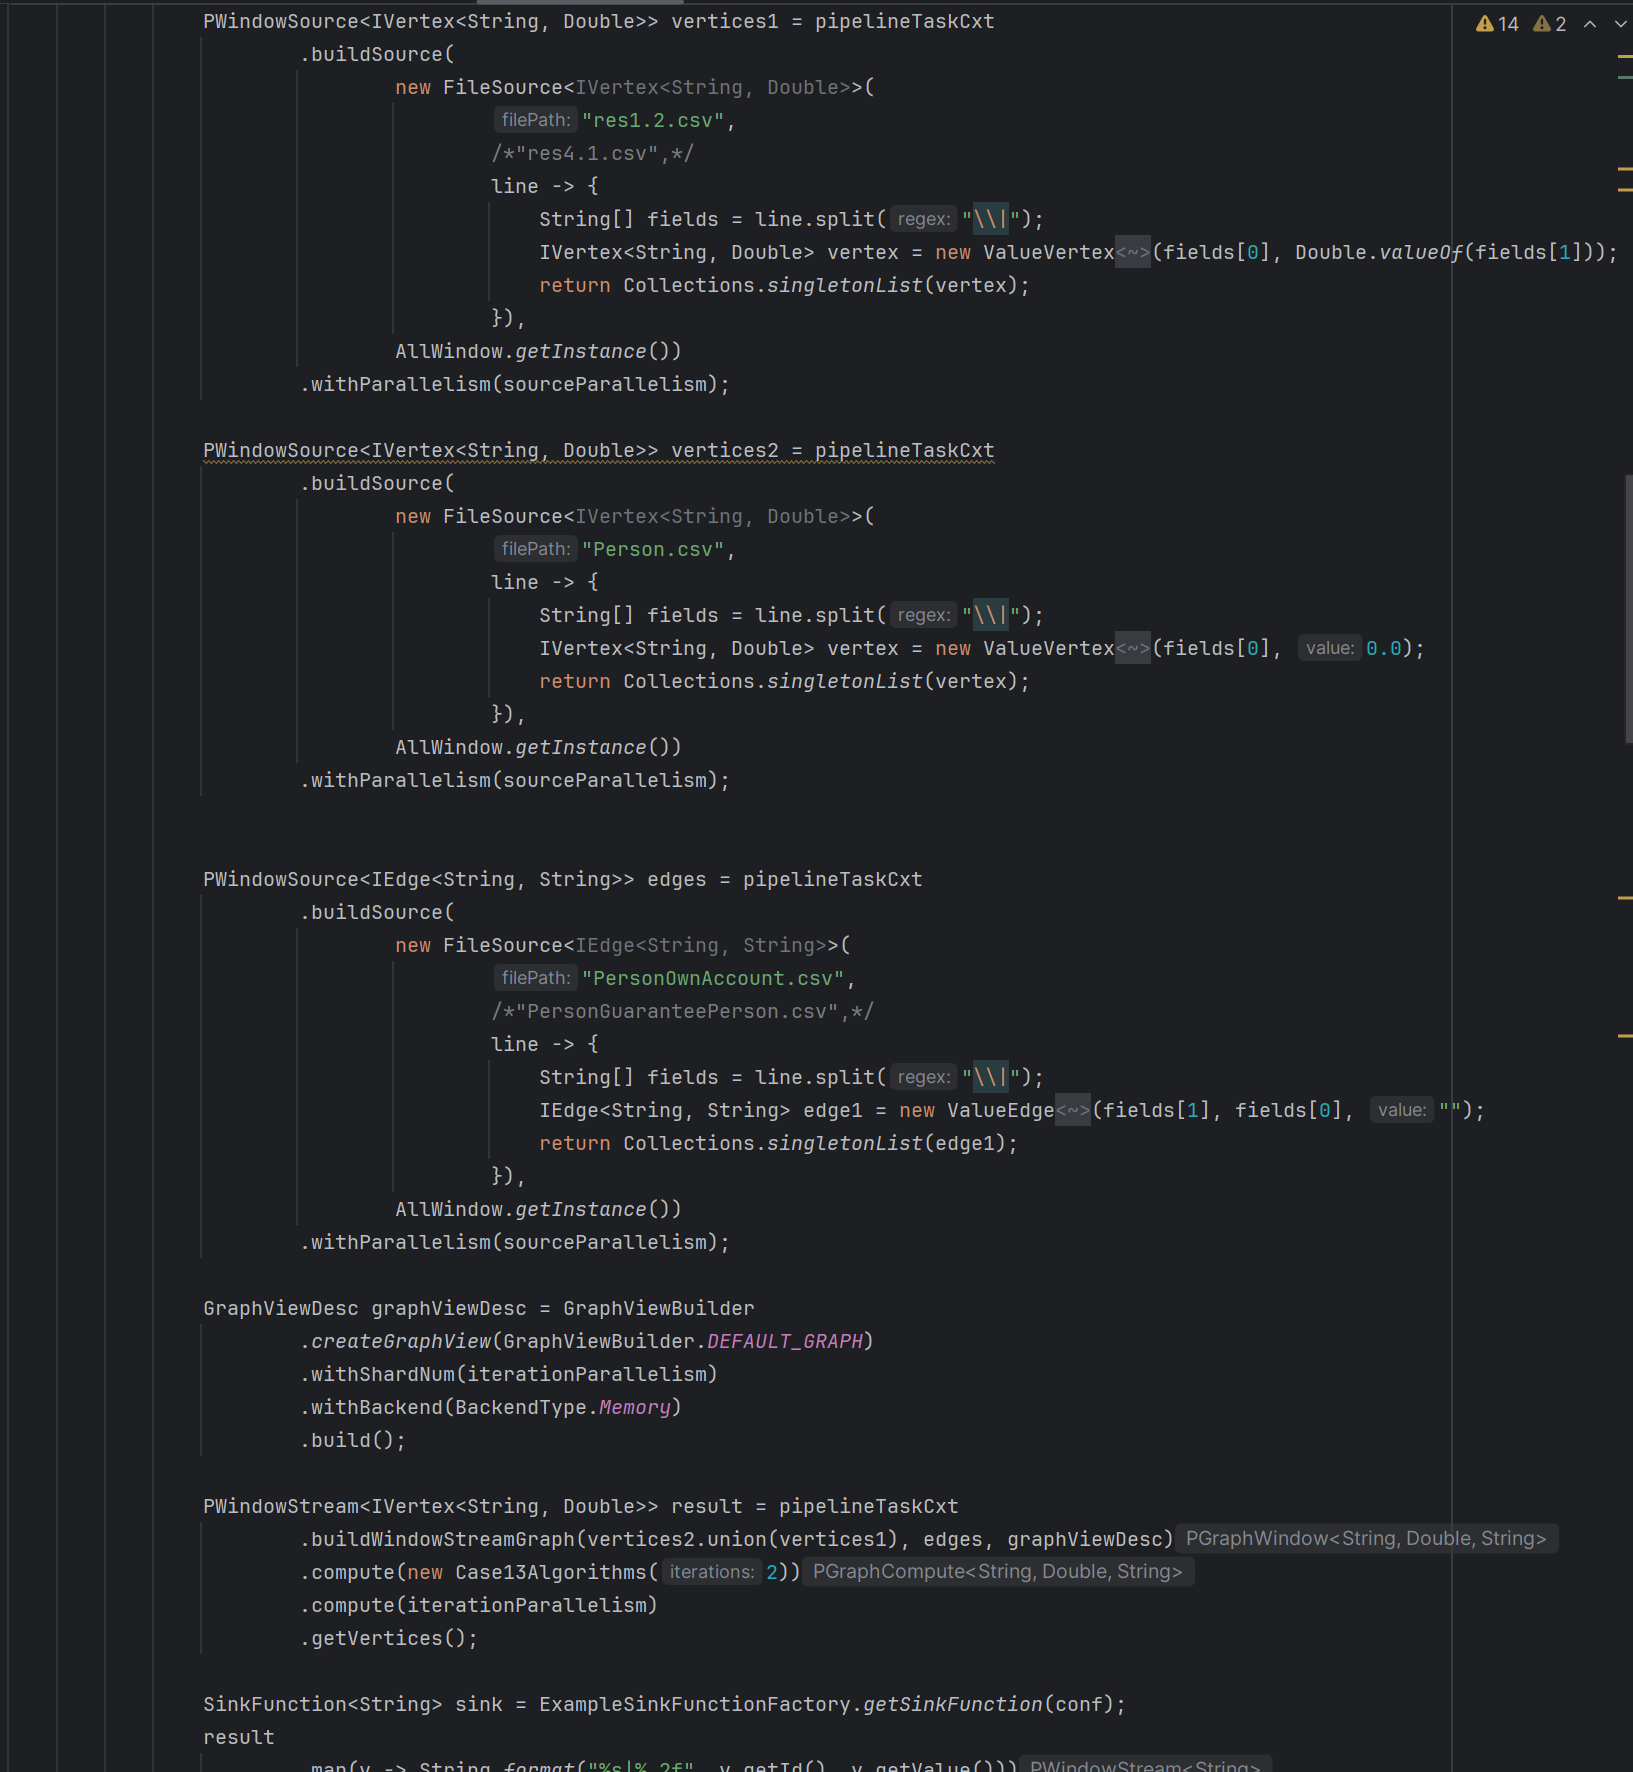
\includegraphics[width=0.85\textwidth,scale=0.7]{./figures/pro4/7.png}
  \end{center}
\end{figure}

接着我们进行两轮迭代,与第二次处理类似,将点的value值根据边往前传递。
不过这次将所有点发送的值为 $ -1 $,用于后续将account点筛选掉。核心代码如下:
\begin{figure}[H]
  \begin{center}
    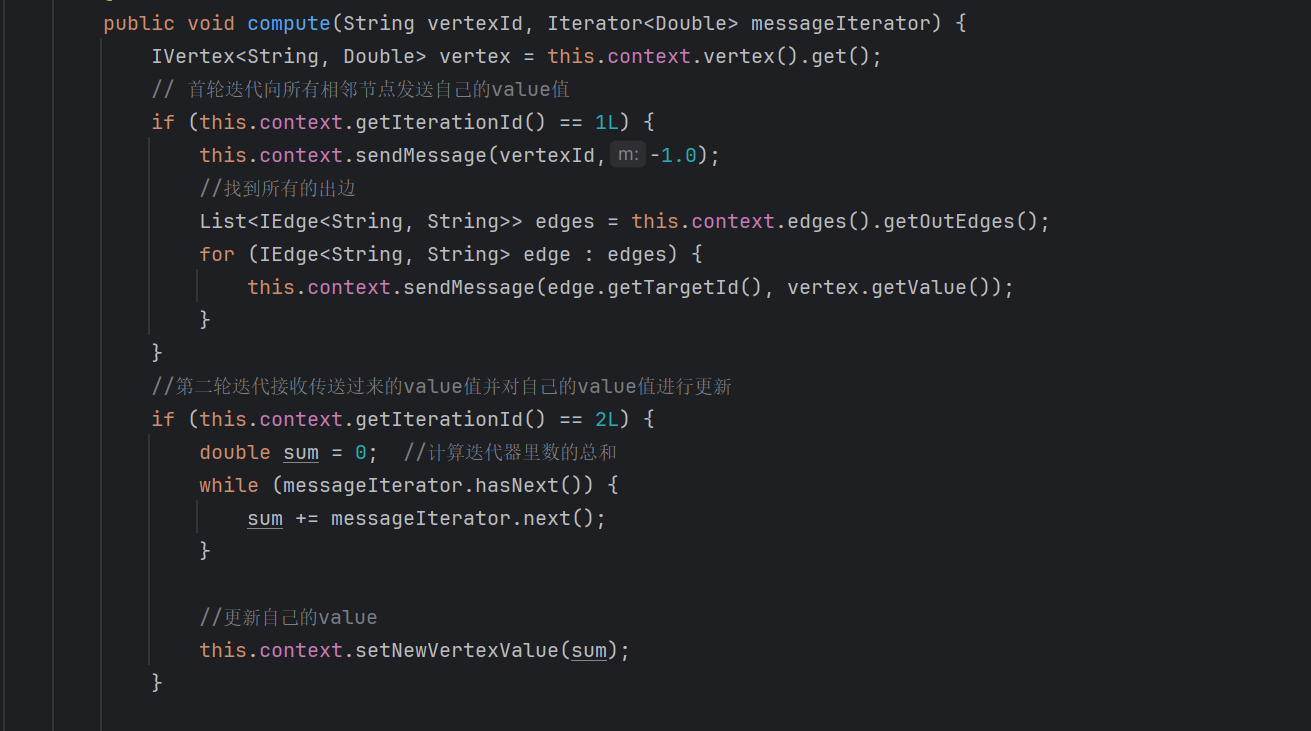
\includegraphics[width=0.85\textwidth,scale=0.7]{./figures/pro4/8.png}
  \end{center}
\end{figure}

最后将结果后保存到文件中
\begin{figure}[H]
  \begin{center}
    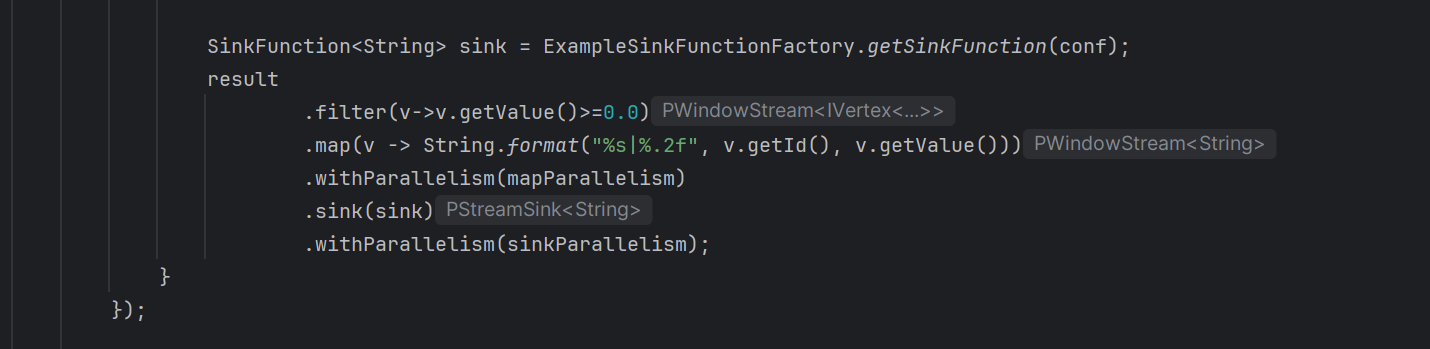
\includegraphics[width=0.85\textwidth,scale=0.7]{./figures/pro4/9.png}
  \end{center}
\end{figure}

但是,提交结果以失败告终了。
我们尝试自己创建文件将自己能想到的所有情况进行测试,结果均正确。但是依然过不了测试,宣告本题以失败告终。但是在尝试过程中也收获了许多知识点。
